\PassOptionsToPackage{svgnames}{xcolor}
\documentclass[a4paper,12pt]{article}

\input preamble.tex

\usepackage{sectsty}
\usepackage{lipsum}
\usepackage{indentfirst}
\allsectionsfont{\centering\normalsize} % Заголовки с абзацного отступа: \indent %% по центру \centering
\subsectionfont{\normalsize\centering} % Подразделы с абзацного отступа + обычный шрифт

\begin{document}
\thispagestyle{empty}
\begin{center}
	Министерство сельского хозяйства РФ \\Федеральное государственное бюджетное образовательное учреждение\\ высшего образования
	\vspace{0.5ex}
	
	<<Пермский государственный аграрно-технологический университет\\ имени академика Д.Н. Прянишникова>>
\end{center}
\vspace{10ex}
\begin{tabularx}{\textwidth}{XX}
	& Кафедра организации аграрного производства \\
%	& территориальной экономики
\end{tabularx}
\begin{center}
	\vspace{13ex}
	Контрольная работа\\
	по дисциплине <<Организация предпринимательской деятельности>> \\
%	\vspace{1ex}
%	на тему <<Экономическая эффективность инвестиционной\\ деятельности предприятия на примере ООО <<Агрофирма Острожка>>
%	\vspace{1ex}
	
%	Вариант 3
\end{center}
	\vspace{8ex}
	\begin{tabularx}{\textwidth}{XX}
	& Выполнил:\\
	& студент факультета заочного \\
	& обучения по направлению \\
	& <<Менеджмент>> \\
	& Кузнецов Андрей Валерьевич \\
	& Шифр Мн-13-204\\
	& Руководитель:\\
	& к.э.н., доцент\\
	& Буторин Сергей Николаевич\\
	\end{tabularx}
\begin{center}
	\vfill
	Пермь 2019
\end{center}

\newpage
%\thispagestyle{empty}
%\begingroup
%	\centering{
		\tableofcontents
				%}
%\endgroup
			
		%

%\newpage
%\subsection*{Введение}
\addcontentsline{toc}{section}{Введение}


\newpage
\section{Стратегические центры хозяйствования как одна из форм управления}

На ранних этапах выработка стратегии начиналась с определения «в какой отрасли работает фирма».
Имелось в виду общепринятое представление о границах, обособлявших фирму и обозначавших внешние пределы для роста и диверсификации, на которые она могла претендовать. Например, Т. Левитт, который в 60-х годах порицал железнодорожные и нефтяные компании за то, что они не смогли определить содержание своей предпринимательской деятельности, предложил им объявить свою отраслевую принадлежность — первым к транспорту, вторым к энергетике.

В глазах тех, кто занимался разработкой стратегии на раннем этапе, определение «отрасли, в которой мы работаем», и выяснение сильных и слабых сторон фирмы было равносильно обозначению границ внимания к традиционным сферам бизнеса.

К началу 60-х годов большинство средних фирм и все без исключения крупные превратились в комплексы, объединяющие выпуск разнородной продукции и выходящие с ней на многочисленные товарные рынки. И если в первой половине века большинство этих рынков росли быстро и сохраняли свою привлекательность, то к началу 60-х годов перспективы их эволюции оказались самыми разными — от бума до упадка. Это расхождение возникло из-за различий в степени насыщения спроса, местных экономических, политических и социальных условиях, конкуренции, темпах обновления технологий.

Становилось всё очевиднее, что продвижение в новые отрасли никоим образом не поможет фирме решить все свои стратегические проблемы или использовать все возможности, так как новые задачи возникали именно в сфере её традиционной деятельности. Поэтому при анализе стратегий в центре внимания всё чаще оказывались перспективы того набора отраслей, которыми фирма уже занималась. Следовательно, первым шагом анализа стало уже не «определение отрасли, в которой работает фирма», а выработка представлений о совокупности тех многочисленных видов деятельности, которыми она занимается.

Это потребовало от управляющих радикально изменить угол зрения. К середине века пришлось научиться видеть перспективы фирмы как бы «изнутри», воспринимая её будущее глазами различных организационных подразделений и с точки зрения традиционных групп товаров, выпускаемых фирмой. Перспективы обычно определялись путём экстраполяции результатов деятельности подразделений фирмы. Однако к началу 70-х годов каждое подразделение обычно обслуживало целую группу рынков с самыми различными перспективами и, в то же время, несколько подразделений могли работать в одной и той же области спроса. Экстраполяция прежних результатов деятельности потеряла свою надёжность и, что важнее всего, не позволяла оценить возможные изменения условий среды во всём их многообразии. Поэтому пришлось научиться «взгляду снаружи», изучать окружение фирмы с точки зрения отдельных тенденций, опасностей, возможностей, которые вытекают из состояния этого окружения.

Единицей такого анализа является стратегическая зона хозяйствования (СЗХ)—отдельный сегмент окружения, на который фирма имеет (или хочет получить) выход. Первый шаг анализа стратегии состоит в определении соответствующих зон, их сследовании вне связей со структурой фирмы или её текущей продукцией. Результатом подобного анализа является оценка перспективы, которая открывается в этой области любому. Достаточно опытному конкуренту с точки зрения роста, нормы прибыли, стабильности и технологии на следующей ступени эта информация необходима для того, чтобы решить, как именно фирма собирается конкурировать с другими фирмами в соответствующей области.

Оценка перспективы с точки зрения внешней среды была впервые предпринята в Министерстве обороны США Р. Макнамарой и Дж. Хитчем, которые разработали принцип раздельных боевых задач — военный эквивалент концепции стратегических зон хозяйствования.

В предпринимательском мире застрельщиком стала американская фирма «Дженерал Электрик», предложившая в дополнение к этой концепции идею стратегического хозяйственного центра (СХЦ)—внутрифирменной организационной единицы, отвечающей за выработку стратегических позиций фирмы в одной или нескольких зонах хозяйствования.

Соотношение понятий стратегической зоны хозяйствования и стратегического хозяйственного центра показано на рис. 2.2.1. Верхняя часть рисунка показывает, что СЗХ характеризуется как определённым видом спроса (потребностей), так и определённой технологией. Например, до 1950 г. потребность в усилении слабых электрических сигналов удовлетворялась посредством технологии электровакуумных ламп. Изобретённый в 1948 г. транзистор стал основой конкуренции в технологии полупроводников.

Потребность в усилении слабых сигналов вместе с полупроводниковой техникой составляет одну СЗХ, перспективы которой после 1950 г. стали угасать. Та же самая потребность плюс транзисторная технология — другая зона, чрезвычайно перспективная в то время.

Как показывает этот пример, едва на смену одной технологии приходит другая, проблема их соотношения становится для фирмы делом важнейшего стратегического выбора: сохранять (и как долго) традиционную технологию или переходить на новую, из-за которой определённая часть продукции, выпускаемой фирмой, оказывается устаревшей. Есть очень много примеров того, как фирмы, не использующие выгоды разработки СЗХ, сохраняют свою прежнюю продукцию даже после того, как она уже устарела.

Рис. 2.2.1. Стратегические зоны хозяйствования и стратегические хозяйственные центры

Как показывает нижняя часть рис. 2.2.1, после выбора СЗХ фирма должна разработать соответствующую номенклатуру изделий. Ответственность за выбор области деятельности, разработку конкурентоспособных изделий и сбытовых стратегий лежит на СХЦ. Как только номенклатура изделий разработана, ответственность за реализацию прибыли ложится на подразделения текущей коммерческой деятельности.

Когда фирма впервые обращается к этой концепции, она должна решить для себя важный вопрос о характере отношений между подразделениями — стратегическими и коммерческими. Например, Макнамара, начав разрабатывать эту концепцию, обнаружил, что главные виды тактических сил — армия, флот, авиация и морская пехота — мешают и зачастую противоречат друг другу в решении раздельных боевых задач стратегического сдерживания, воздушной обороны Соединённых Штатов, ограниченных военных действий и т д. Решение Макнамары состояло в создании новых подразделений, которые занимаются стратегическим планированием соответствующих раздельных задач. Разработанные ими стратегические решения передаются «через дорогу» — соответствующим департаментам для реализации. Таким образом, по замыслу Макнамары, стратегические подразделения отвечали только за разработку планируемой стратегии, а департаменты — за её реализацию. Это разделение вызвало разнобой и потерю координации, в частности, из-за того, что некоторые департаменты зачастую выполняли обязанности стратегических подразделений. Так, например, ответственными за разработку отдельных функций стратегического сдерживания оказались одновременно и военно-морской флот, и военная авиация.

Чтобы избежать такой двойной стратегической ответственности, фирма «Дженерал Электрик» нашла другой вариант решения. Она проделала нелёгкую работу — распределила свои отделения текущей коммерческой деятельности (группы заводов, КБ, сбытовые конторы и т. д. — Прим. науч. ред.) между СХЦ с тем, чтобы последние отвечали не только за планирование и реализацию стратегии, но и за конечный результат — получение прибыли.

Такой подход позволил избавиться от передачи стратегии «через дорогу» и возложил на СХЦ ответственность и за прибыли, и за убытки. Тем не менее, как обнаружила «Дженерал Электрик» и другие компании, сложившаяся организационная структура не в полной мере соответствует вновь созданным СХЦ, в силу чего не представляется возможным разделить ответственность чётко и однозначно.

Третий вариант решения состоит в реорганизации фирмы на базе СХЦ с тем, чтобы каждому из них соответствовало одно подразделение текущей коммерческой деятельности. Этот вариант, на первый взгляд такой простой, имеет свои трудности, так как главный критерий образования СХЦ внутри организации — эффективность развития по данному стратегическому направлению — является только одним из определяющих параметров организационной структуры в целом. Есть и другие: эффективное использование технологии и высокий уровень рентабельности. Реорганизация на базе СХЦ, максимизируя эффективность стратегического поведения, может в то же время снизить показатели рентабельности фирмы или просто оказаться невыполнимой задачей в силу каких-либо причин, связанных с технологией (в гл. 4.3. мы рассмотрим проблему согласования стратегических разработок с текущей деятельностью в рамках организационной структуры).

Из вышеизложенного видно, что проблема распределения ответственности между СХЦ фирмы отнюдь не проста и её решение может быть каждый раз иным. Тем не менее, уже достаточно хорошо известно из опыта, что концепция СЗХ и СХЦ — это необходимый инструмент, обеспечивающий фирме ясное представление о том, каким может стать в будущем её окружение, что чрезвычайно важно для принятия эффективных стратегических решений.
%\input{1-3glava}

%\newpage
%\section{Управление рисками предприятия, методы оценки рисков}

Управление рисками --- это процессы, связанные с идентификацией, анализом рисков и принятием решений, которые включают максимизацию положительных и минимизацию отрицательных последствий наступления рисковых событий. Процесс управления рисками проекта обычно включает выполнение процедур, приведенных на рисунке \ref{fig:diagram-page-2}.

\begin{figure}[!h]
	\centering
	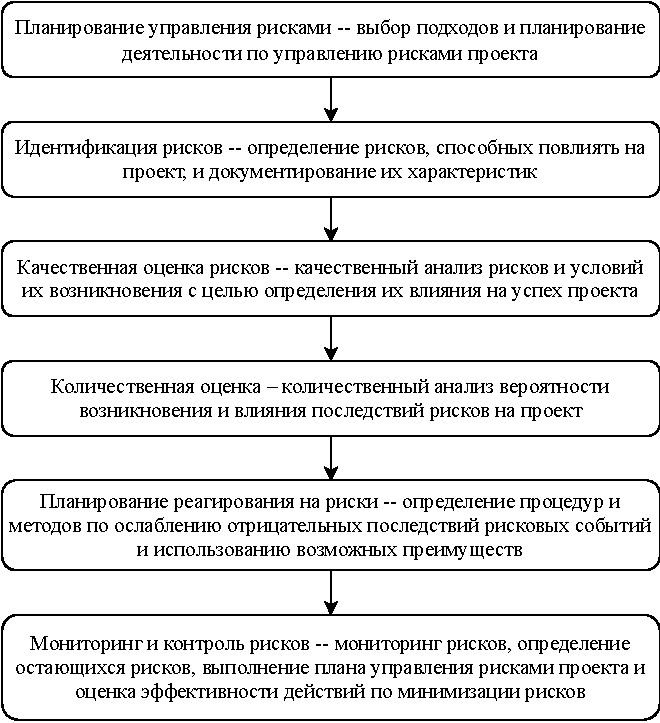
\includegraphics[width=0.7\linewidth]{Diagram-Page-2}
	\caption{Этапы управления рисками проекта}
	\label{fig:diagram-page-2}
\end{figure}

Планирование управления рисками --- процесс принятия решений по применению и планированию управления рисками для конкретного проекта. Этот процесс может включать в себя решения по организации, кадровому обеспечению процедур управления рисками проекта, выбор предпочтительной методологии, источников данных для идентификации риска, временной интервал для анализа ситуации. Важно спланировать управление рисками, адекватное как уровню и типу риска, так и важности проекта для организации.

Идентификация рисков --- заключается в систематическом выявлении рисков, характерных для определенного вида деятельности, и определении их характеристик.

Идентификация сводится к выявлению возможных проблем. 
Под «проблемой» понимают что-либо (событие, объект, человека, идею), что может встать между организацией и ее целями.
Необходимо определить, что пойдет «не так», чтобы затем решить, как это устранить или обойти.

Идентификация риска --- процесс нахождения, составления перечня и описания элементов риска.
Основные элементы риска:
\begin{itemize}
\item  – причины, приводящие к наступлению опасного явления;
\item – опасные явления (события), оказывающие воздействие на объ-
ект;
\item – виды воздействия, которые могут привести к изменению со-
стояния объекта;
\item – последствия, представляющие собой потери из-за воздействия,
и их оценку со стороны субъекта;
\item – факторы риска, влияющие на вероятность реализации риска
и тяжесть последствий.
\end{itemize}


%\newpage
%\section{Основные причины сопротивления изменениям}



%\newpage
%\section{Задачи}
\subsection{Задача 1}
%\nocite{michurina,01,02,03,04,05,06,07,08,09,10}

\newpage
\renewcommand\refname{Список использованных источников}
\addcontentsline{toc}{section}{Список использованных источников}
\printbibliography
%\addcontentsline{toc}{section}{Приложения}
%\small{\listoftables}
%\addcontentsline{toc}{section}{Список таблиц}
%\newpage
%\thispagestyle{empty}
%\topskip0pt
%\vspace*{\fill}%
%\begin{center}
%	\textbf{ПРИЛОЖЕНИЯ}
%\end{center}
%\vspace*{\fill}
%
\end{document}
